% !TeX spellcheck = it_IT
\section{Introduzione all'High Performance Computing HPC}

L'uso delle GPU permette di incrementare significativamente le performance, per avere speed-up anche nell'ordine delle migliaia, per problemi altamente parallelizzabili. Si parlerà di paradigma \textbf{GP-GPU} (\textbf{General Purpose - GPU}).

Esistono molti sistemi che si basano su operazioni semplici ma ripetute numerose volte. Esempio: il prodotto matriciale è il prodotto vettore-vettore ripetuto. Questi sistemi sono facilmente parallelizzabili (se non ci sono interdipendenze tra i risultati).

\paragraph{Parallelismo:} Vogliamo accelerare il tempo, il parallelismo è la capacità di eseguire parti di un calcolo in modo concorrente. Esistono problemi che sarebbero impensabili senza l'accelerazione permessa dal parallelismo. Permette di risolvere problemi più grandi nello stesso tempo, o problemi di dimensione fissa in tempo più breve.

Il parallelismo sarà gestito a livello di \textbf{thread}: unità di esecuzione costituita da una sequenza di istruzioni e gestita dal sistema operativo o da un sistema di runtime.

\paragraph{Paradigma GP-GPU:} Fa riferimento all'uso di GPU (Graphics Processing Unit) per eseguire computazioni di carattere generale, di qualsiasi tipo. Implica l'uso di CPU e GPU in maniera congiunta, la computazione parte comunque dalla CPU (chiamata \textbf{host}) la quale effettuerà richieste alla GPU (chiamata \textbf{device}), quest'ultima diventa un coprocessore. Viene separata la parte sequenziale dell'applicazione e di controllo, che va sulla CPU, dalla parte a maggior intensità computazionale, lasciata alla GPU.

La GPU non è una piattaforma stand-alone, ma è un coprocessore che opera congiuntamente alla CPU, comunicando tramite bus PCI-Express. Sono necessari trasferimenti e la CPU orchestra la "sincronizzazione".
\begin{center}
	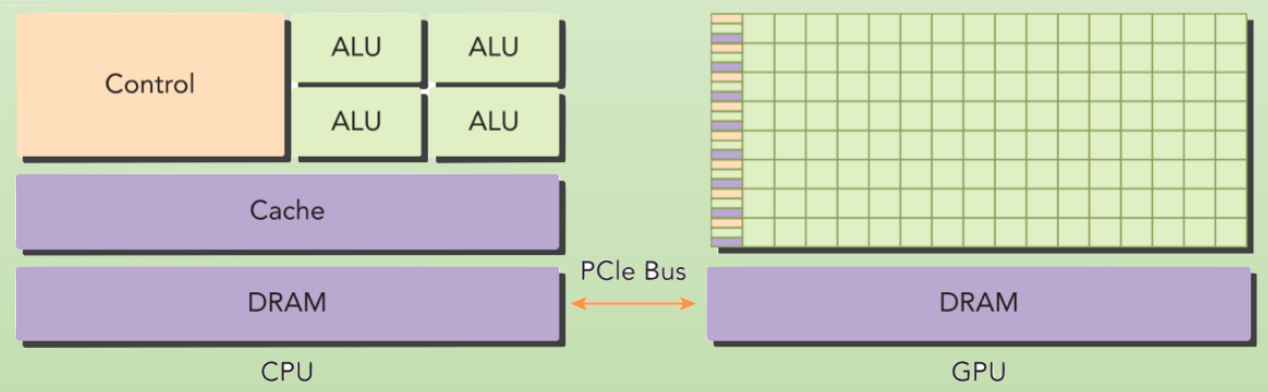
\includegraphics[width=0.95\linewidth]{img/intro/gpgpu1}
\end{center}

L'uso, dal punto di vista dell'utente, di un sistema con GPU è \textbf{trasparente}, si ha un risultato più veloce ma dall'esterno non cambia l'esperienza.

Le funzioni vanno riscritte in modo da poterle esporre al parallelismo sulla GPU. I "\textbf{kernel}" sono le funzioni demandate alla GPU.  Le applicazioni ibride avranno parti di codice host, eseguito sulla CPU, e parti di codice device, eseguito sulla GPU. 

La CPU si occupa della gestione dell'ambiente, dei dati per il device stesso ed è ottimizzata per tutte le sequenze di operazioni con un flusso di controllo impredicibile, mentre la GPU è ideale per flussi di controllo semplici.

Un problema da considerare è l'uso di energia: si vuole massimizzare la potenza di calcolo minimizzando l'energia consumata.

La differenza di esecuzione è
\begin{itemize}
	\item CPU: pochi core ottimizzati per l'elaborazione sequenziale
	\item GPU: architettura massicciamente parallela che consiste di migliaia di core che cooperano in modo efficiente per trattare molteplici task in maniera concorrente
\end{itemize}

Il calcolo parallelo può essere realizzato in vari modi, tra cui: 
\begin{itemize}
	\item parallelismo nei \textbf{dati}: suddivisone dei dati in parti uguali per essere elaborati simultaneamente su più processori
	\item parallelismo sui \textbf{task}: il lavoro viene suddiviso in attività indipendenti ed ogni task viene eseguito dal suo processore. Nel processo di parallelizzazione bisogna tenere in considerazione le dipendenze tra i task
	\item parallelismo di \textbf{istruzioni}: un programma viene diviso in istruzioni ed ognuna di queste parti indipendenti viene eseguita simultaneamente su più processori
\end{itemize}
L'ambito di utilizzo del parallelismo dato dalle GPU è con \textbf{dimensioni dei dati abbastanza ampie} che allo stesso tempo permettono buon parallelismo.

\paragraph{Tassonomia di Flynn:} I modelli di computazione fondamentali sono: 
\begin{itemize}
	\item \textbf{SISD Single Instruction Single Data:} una unità che esegue una operazione (sequenziale); questo è il modello di Von Neumann
	
	\item \textbf{SIMD Single Instruction Multiple Data:} una singola istruzione per molteplici unità di calcolo, applicata su molti dati
	
	\item \textbf{MISD Multiple Instruction Single Data:} il parallelismo è solo a livello di istruzioni, molte unità sugli stessi dati; non ha implementazioni realistiche
	
	\item \textbf{MIMD Multiple Instruction Multiple Data:} molteplici unità che possono accedere a molteplici dati, ognuna con istruzioni proprie
\end{itemize}

\paragraph{SIMT Model:} Modello Single Instruction Multiple Thread, introdotto da CUDA. Ogni thread ha la possibilità di "scegliere una strada" in base al dato. Il flusso di controllo parallelo parte assieme ma può portare a branch differenti, in base ai dati. Estende il concetto di SIMD permettendo flussi individuali per ogni thread, con il costo relativo a gestire la decisione locale sui thread (program counter e registri).
\label{par:simt}

\subsection{Architettura Nvidia}

\paragraph{Streaming Multiprocessor SM:} Le GPU sono costituite di array di SM, ognuno dei quali composto da gruppi di 32 CUDA core, chiamati \textbf{warp}. Ogni SM in una GPU è progettato per supportare l'esecuzione concorrente di centinaia di thread. In un warp tutti i thread dovrebbero essere SIMD, ovvero eseguire la stessa istruzione allo stesso tempo.

Questo è il modello iniziale, nel tempo si è evoluto aggiungendo elementi come una gerarchia di cache migliorata, altri core dedicati ad applicazioni specifiche (ad esempio, i tensor core per il calcolo matriciale). Ogni CUDA core ha i suoi registri e unità di calcolo (FP e INT).

\paragraph{Compute Capability CC:} Rappresenta la versione dell'architettura CUDA supportata da una GPU Nvidia. Definisce le funzionalità hardware disponibili, come il numero di core CUDA, il supporto per le istruzioni avanzate, uso della memoria, risorse, ecc. Viene usato in fase di compilazione per determinare l'architettura per cui compilare.

\paragraph{CUDA Toolkit:} Fornisce tutti gli strumenti per la programmazione in CUDA C/C++ (e oltre). Permette compilazione, profilazione e debugging, assieme a librerie ecc.; tutto ciò che serve per sviluppare.

\paragraph{CUDA APIs:} Sono presenti due livelli di API per la gestione della GPU e l'organizzazione dei thread:
\begin{itemize}
	\item \textbf{CUDA Runtime API}
	\item \textbf{CUDA Driver API}
\end{itemize}
Le driver API sono API a basso livello e piuttosto difficili da programmare ma danno un maggior controllo della GPU.

Runtime porta una astrazione maggiore, per un utilizzo più user-friendly ma richiede di compilare con \texttt{nvcc} e dipendono dalla versione del driver. Le funzioni cominciano con il nome "\texttt{cuda}".